\section{Thực nghiệm}

\subsection{Thiết lập thực nghiệm}
\textbf{Bộ dữ liệu.} Chúng tôi tiến hành các thí nghiệm trên ba bộ dữ liệu benchmark cho zero-shot learning, đó là CUB \cite{49}, AwA2 \cite{29}, SUN \cite{38}. Cụ thể, CUB chứa 11,788 hình ảnh trên 200 loài chim, mỗi loài được chú thích với 312 thuộc tính. AwA2 bao gồm 37,322 hình ảnh trên 50 loài động vật được mô tả bởi 85 thuộc tính. SUN bao gồm 14,340 hình ảnh từ 717 lớp cảnh được chụp với 102 thuộc tính. Chúng tôi sử dụng các phân chia huấn luyện được đề xuất trong \cite{60}, các lớp đã thấy/chưa thấy được chia thành 150/50, 40/10 và 645/72 tương ứng.

\textbf{Đánh giá.} Theo \cite{59}, chúng tôi đo lường độ chính xác top-1 trong cả hai cài đặt zero-shot learning (ZSL) và generalized zero-shot learning (GZSL). Trong cài đặt ZSL, chúng tôi chỉ đánh giá độ chính xác của các mẫu thử nghiệm trong các lớp chưa thấy. Trong cài đặt GZSL, chúng tôi tính toán độ chính xác của các mẫu thử nghiệm từ cả hai lớp đã thấy (ký hiệu là S) và chưa thấy (ký hiệu là U). Để đánh giá hiệu suất chung, trung bình điều hòa (harmonic mean) giữa các lớp đã thấy và chưa thấy là một số liệu đánh giá chính trong cài đặt GZSL, được định nghĩa là $H = (2 \times S \times U) / (S + U)$.

\textbf{Triển khai.} Mô hình của chúng tôi được triển khai dựa trên mô hình ViT-base \cite{47} (kích thước đầu vào hình ảnh: 224$\times$224), được huấn luyện trước trên ImageNet-1k làm cơ sở và để khởi tạo, điều này nhất quán với các phương pháp ZSL dựa trên ViT hiện có. ViT-base có số lượng bản vá mặc định là 196, nhưng để hiệu quả tính toán, chúng tôi tổng hợp mỗi 4 (2$\times$2) bản vá thành một, cho ra 49 bản vá.

\subsection{Kết quả chính}
\textbf{Hiệu quả đối với sự sai lệch ngữ nghĩa.} Để cho thấy hiệu quả của SVIP trong việc giải quyết sự sai lệch ngữ nghĩa, chúng tôi so sánh SVIP với các phương pháp nhằm đạt được điều này trong không gian đặc trưng (RFF \cite{27}, SDGZSL \cite{9}, Dis-VAE \cite{30}) hoặc ở cấp độ mô hình (ZSLViT \cite{4}). Như được trình bày trong Bảng 1, phương pháp của chúng tôi đạt được hiệu suất vượt trội trong cả hai cài đặt ZSL và GZSL trên ba bộ dữ liệu benchmark, ngoại trừ hiệu suất ZSL trên AwA2 mà chúng tôi đạt được hiệu suất tương đương. Những cải tiến này xác nhận rằng việc lọc các bản vá không liên quan ở giai đoạn đầu vào là rất hiệu quả để tăng cường sự liên kết thị giác-ngữ nghĩa và nâng cao độ chính xác nhận dạng zero-shot tổng thể.

\textbf{So sánh với các Backbone CNN.} Tiếp theo, chúng tôi so sánh SVIP với một nhóm các phương pháp sử dụng ResNet101 làm backbone của chúng (khối trên của Bảng 1). Cụ thể, các phương pháp như APN \cite{61}, GEM \cite{33}, MSDN \cite{3}, Dis-VAE, và ICCE đều hoạt động trên các đặc trưng toàn cục được trích xuất từ CNN để căn chỉnh không gian thị giác và ngữ nghĩa cho zero-shot learning. Mặc dù chúng có hiệu quả trên một số bộ dữ liệu nhất định, SVIP của chúng tôi đạt được kết quả hiệu suất hiện đại một cách nhất quán trên CUB, AwA2 và SUN. Đáng chú ý, SVIP đạt được giá trị H là 75.0\% trên CUB, 74.9\% trên AwA2 và 50.7\% trên SUN, vượt qua tất cả các phương pháp dựa trên ResNet101 cạnh tranh. Những kết quả này chứng tỏ hiệu quả của SVIP trong việc nắm bắt các tín hiệu ngữ nghĩa chi tiết trong khi vẫn duy trì khả năng phân biệt mạnh mẽ cho cả các lớp đã thấy (S) và chưa thấy (U).

\textbf{So sánh với các Backbone ViT.} Tiếp theo, chúng tôi so sánh SVIP với các phương pháp gần đây với ViT làm backbone, bao gồm các phương pháp dựa trên ngôn ngữ (CLIP \cite{41}, CoOp \cite{72}, I2DFormer \cite{34}, I2MV \cite{35}), các phương pháp dựa trên thuộc tính (DUET \cite{13}, ZSLViT \cite{4}). Nói chung, các phương pháp dựa trên ViT được hưởng lợi từ các cơ chế chú ý trên các nhúng bản vá, nhưng chúng thường thiếu sự giám sát rõ ràng cho các bản vá không liên quan đến ngữ nghĩa. Như đã trình bày, SVIP mang lại hiệu suất tốt nhất về độ chính xác chưa thấy (U) trên CUB (72.1\%) và SUN (53.7\%), cũng như trung bình điều hòa hàng đầu trên cả hai bộ dữ liệu. Trên AwA2, phương pháp của chúng tôi cũng cho thấy kết quả cạnh tranh, chứng tỏ khả năng thích ứng của lý luận thuộc tính cục bộ của SVIP trên một loạt các miền thị giác.

\textbf{Nghiên cứu cắt bỏ (Ablation Study).} Chúng tôi tiến hành một nghiên cứu cắt bỏ để phân tích sự đóng góp của từng thành phần trong SVIP (Bảng 2). Baseline (ViT) sử dụng một lớp tuyến tính đơn giản trên token lớp mà không có các hoạt động cấp bản vá, mang lại hiệu suất thấp nhất. SVIP không có SSPS loại bỏ Lựa chọn bản vá Tự giám sát, áp dụng các bản vá ngữ nghĩa một cách bừa bãi, dẫn đến sụt giảm đáng kể, làm nổi bật sự cần thiết của việc lựa chọn bản vá có mục tiêu. SVIP không có PSC loại bỏ trực tiếp các bản vá không liên quan đến ngữ nghĩa thay vì bối cảnh hóa chúng, điều này làm gián đoạn một chút cấu trúc đối tượng và làm giảm hiệu suất. SVIP không có JSD loại trừ phân kỳ Jensen-Shannon, làm giảm sự ổn định huấn luyện và độ chính xác tổng thể. SVIP không có W2P thay thế các nhúng từ bằng các nhúng bản vá được khởi tạo ngẫu nhiên, dẫn đến sự suy giảm liên kết ngữ nghĩa. SVIP không có P2A loại bỏ ánh xạ Patch-to-Attribute, buộc phải dựa vào token lớp, điều này làm suy yếu độ chính xác của lớp chưa thấy.

\textbf{Độ nhạy của siêu tham số.} Trong một loạt các thí nghiệm, chúng tôi khảo sát ảnh hưởng của bốn siêu tham số đến hiệu suất của phương pháp được đề xuất của chúng tôi. Hình \ref{fig:hyperparameter} (a) cho thấy ảnh hưởng của việc thay đổi số lượng bản vá được bảo tồn M từ 49 đến 35. Hiệu suất bão hòa xảy ra ở khoảng 40, và số lượng bản vá lớn hơn có xu hướng làm giảm hiệu suất do cắt tỉa quá mức các bản vá liên quan đến ngữ nghĩa. Hình \ref{fig:hyperparameter} (b) chứng minh rằng Phân kỳ JS là một siêu tham số khá nhạy cảm, đạt hiệu suất tốt nhất ở mức 1. Trong Hình \ref{fig:hyperparameter} (c), chúng tôi thay đổi hệ số mất mát cho bộ phân loại bản vá $\lambda_2$ và thấy rằng cả ZSL và GZSL đều đạt hiệu suất tốt nhất ở mức 3. Trong Hình \ref{fig:hyperparameter} (d), chúng tôi thấy rằng thang nhiệt độ có tác động đáng kể đến sự thay đổi hiệu suất, đạt đỉnh ở mức 5.

\begin{table*}[t]
    \centering
    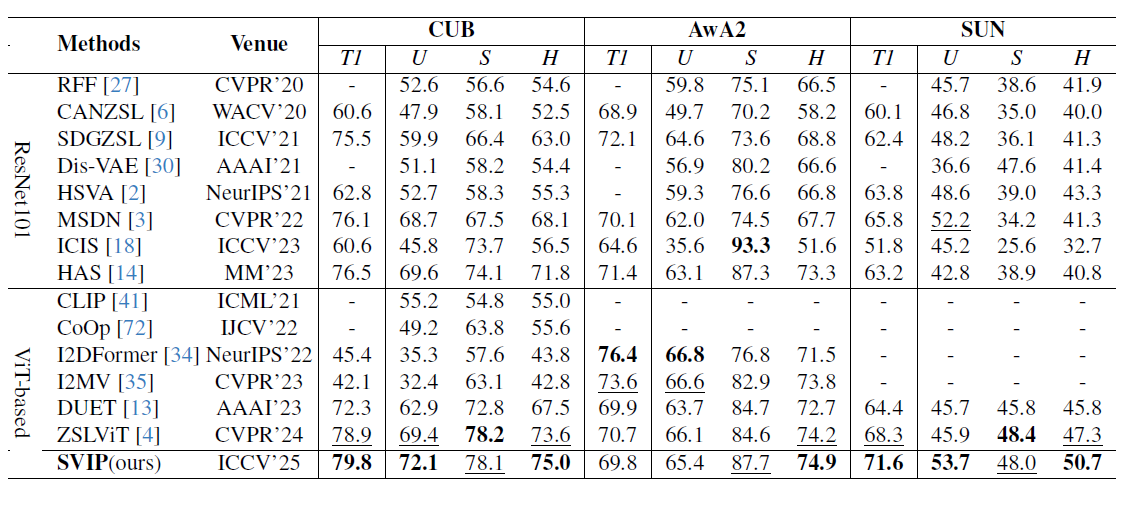
\includegraphics[width=\textwidth]{Image/Table 1.PNG}
    \caption{So sánh các mô hình ZSL và GZSL hiện đại trên ba bộ dữ liệu benchmark. Đối với ZSL, kết quả được báo cáo là độ chính xác top-1 trung bình (T1). Đối với GZSL, chúng tôi báo cáo độ chính xác top-1 cho các lớp chưa thấy (U) và đã thấy (S), cùng với trung bình điều hòa của chúng (H). Các kết quả tốt nhất và tốt thứ hai được tô đậm và gạch chân, tương ứng.}
    \label{tab:main_results}
\end{table*}

\begin{table*}[t]
    \centering
    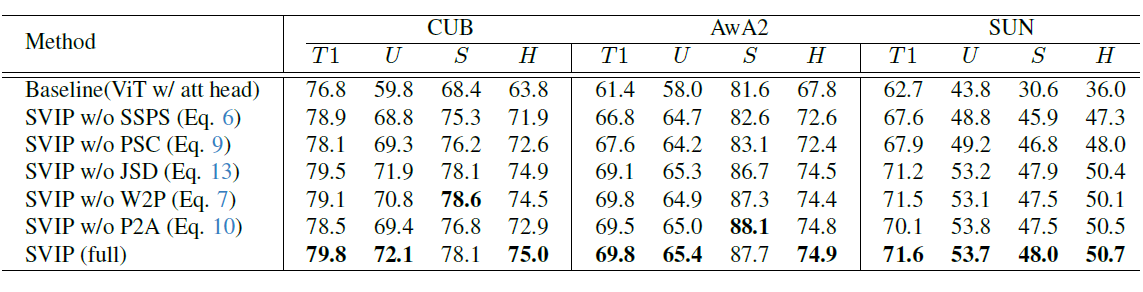
\includegraphics[width=\textwidth]{Image/Table 2.PNG}
    \caption{Phân tích các thành phần khác nhau trong SVIP.}
    \label{tab:ablation}
\end{table*}

\begin{figure*}[t]
    \centering
    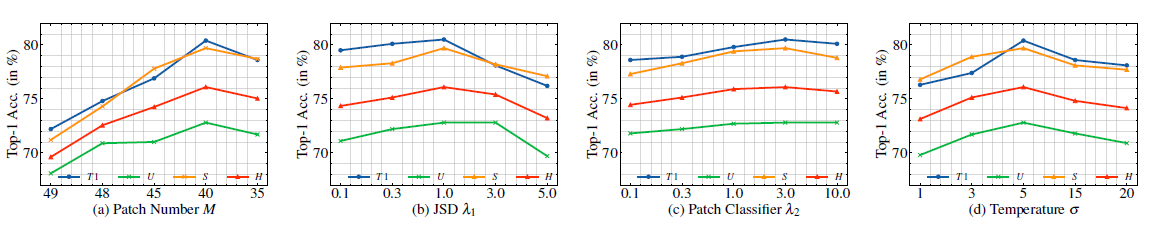
\includegraphics[width=\textwidth]{Image/Figure 4.PNG}
    \caption{Độ nhạy của siêu tham số trên bộ dữ liệu CUB. Trục ngang chỉ ra các siêu tham số thay đổi cho (a) số lượng bản vá được bảo tồn M, (b) hệ số mất mát JSD $\lambda_1$, (c) hệ số mất mát bộ phân loại bản vá $\lambda_2$, và (d) nhiệt độ logits $\sigma$.}
    \label{fig:hyperparameter}
\end{figure*}

\subsection{Nghiên cứu Định tính}
\textbf{Cục bộ hóa Thuộc tính (Attribute Localization).} Chúng tôi trình bày các bản đồ chú ý (tức là, lớp trước hoạt động gộp tối đa) trong Hình \ref{fig:attention_maps}, cho các thuộc tính được chọn ngẫu nhiên trên ba hình ảnh ví dụ từ bộ dữ liệu CUB. Các bản đồ chú ý được tạo ra bằng cách áp dụng các hoạt động gộp tối đa cho đầu ra của mô hình, làm nổi bật các vùng mà mô hình đang tập trung vào cho mỗi thuộc tính. Các vùng được che bằng sọc chéo được xác định là các bản vá không liên quan đến ngữ nghĩa và do đó không được xem xét để cục bộ hóa thuộc tính. Phương pháp cơ sở ViT tập trung vào nhiều bản vá không chính xác được phân loại là các bản vá không liên quan đến ngữ nghĩa trong SVIP, điều này chứng tỏ sự hữu ích của SSPS.

\textbf{Trực quan hóa Dự đoán Thuộc tính.} Hình \ref{fig:tsne_visualization} trình bày một trực quan hóa t-SNE của các véc-tơ thuộc tính được dự đoán từ ViT cơ sở (trái) và SVIP được đề xuất của chúng tôi (phải) trên các hình ảnh của 20 lớp được chọn ngẫu nhiên từ tập hợp chưa thấy của bộ dữ liệu CUB. Trong ViT cơ sở Hình \ref{fig:tsne_visualization}(a), các cụm xuất hiện kém khác biệt hơn, với các điểm thuộc tính chồng chéo và phân tán, như được chỉ ra bởi các vòng tròn đứt nét màu đỏ. Điều này cho thấy rằng thông tin không liên quan đến ngữ nghĩa làm gián đoạn các biểu diễn đã học, dẫn đến sự liên kết thị giác-ngữ nghĩa yếu hơn. Ngược lại, SVIP trong Hình \ref{fig:tsne_visualization}(b) cho thấy các cụm nhỏ gọn và được phân tách rõ ràng hơn, trong đó các thuộc tính được phân định rõ ràng hơn. Các vòng tròn đứt nét màu đỏ làm nổi bật cách SVIP giảm sự mơ hồ về ngữ nghĩa, đảm bảo rằng các thuộc tính tương tự tạo thành các nhóm mạch lạc và có cấu trúc tốt hơn. Những kết quả này xác thực hiệu quả của việc lựa chọn bản vá tự giám sát và bối cảnh hóa ngữ nghĩa trong việc cải thiện.

\textbf{Trực quan hóa Đặc trưng của Bộ phân loại Bản vá.} Hình \ref{fig:patch_visualization} minh họa cách phương pháp của chúng tôi lựa chọn và bối cảnh hóa các bản vá không liên quan đến ngữ nghĩa. Trong (a), mỗi hình ảnh chim được phân vùng thành các bản vá, và những bản vá được coi là không liên quan sẽ được tô bóng (sọc chéo). Việc lọc ở giai đoạn đầu này đảm bảo rằng mô hình tập trung vào các thuộc tính quan trọng để nhận dạng chim (ví dụ: các mẫu màu hoặc hình dạng đặc biệt). Trong (b), chúng tôi sử dụng t-SNE để trực quan hóa các nhúng trong lớp trung gian của bộ phân loại bản vá trong không gian hai chiều. Chúng tôi quan sát thấy rằng các bản vá không liên quan đến ngữ nghĩa cụm lại với nhau như được chỉ ra trong các hộp giới hạn màu đỏ, trong khi các bản vá ghi lại các đặc điểm có liên quan về mặt ngữ nghĩa thì phân tán hơn. Sự tách biệt này chứng thực khả năng của bộ phân loại bản vá của chúng tôi trong việc bảo tồn các tín hiệu thị giác có ý nghĩa và triệt tiêu thông tin không liên quan.

\begin{figure*}[t]
    \centering
    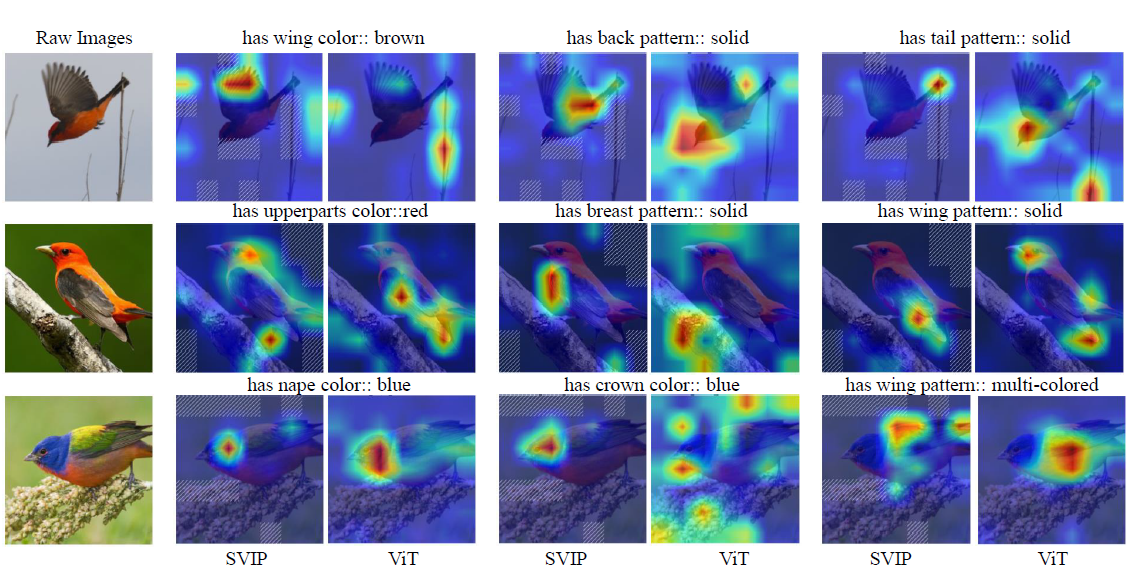
\includegraphics[width=\textwidth]{Image/Figure 5.PNG}
    \caption{Trực quan hóa các bản đồ chú ý thuộc tính được dự đoán trên ba mẫu thử nghiệm ngẫu nhiên của bộ dữ liệu CUB.}
    \label{fig:attention_maps}
\end{figure*}

\begin{figure*}[t]
    \centering
    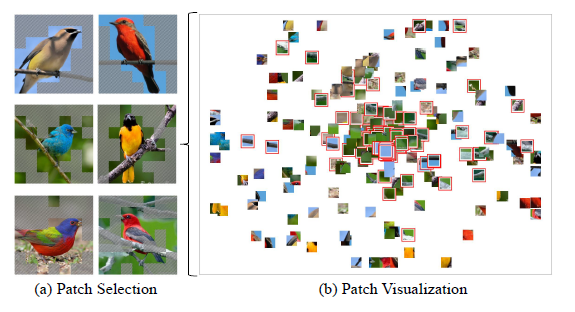
\includegraphics[width=\textwidth]{Image/Figure 6.PNG}
    \caption{(a) Hình ảnh ví dụ với các bản vá không liên quan đến ngữ nghĩa được che. (b) Trực quan hóa t-SNE của các bản vá hình ảnh, trong đó các hộp giới hạn màu đỏ chỉ ra các bản vá không liên quan về mặt ngữ nghĩa.}
    \label{fig:patch_visualization}
\end{figure*}

\begin{figure*}[t]
    \centering
    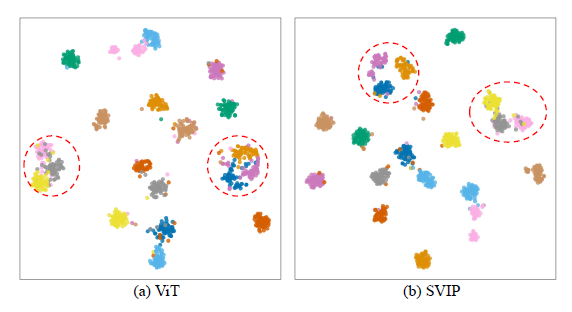
\includegraphics[width=0.9\textwidth]{Image/Figure 7.PNG}
    \caption{Trực quan hóa t-SNE của các véc-tơ thuộc tính được dự đoán từ (a) ViT cơ sở và (b) SVIP được đề xuất của chúng tôi.}
    \label{fig:tsne_visualization}
\end{figure*}
